\documentclass{article}

\usepackage[preprint]{agents4science_2025}

\usepackage[utf8]{inputenc}
\usepackage[T1]{fontenc}
\usepackage{hyperref}
\usepackage{url}
\usepackage{booktabs}
\usepackage{amsfonts}
\usepackage{nicefrac}
\usepackage{microtype}
\usepackage{xcolor}
\usepackage{graphicx}
\usepackage{amsmath}
\usepackage{array}
\usepackage{multirow}
\usepackage{listings}
\usepackage{float}

\lstset{
    language=C,
    basicstyle=\footnotesize\ttfamily,
    keywordstyle=\color{blue}\bfseries,
    commentstyle=\color{green!60!black},
    numberstyle=\tiny\color{gray},
    numbers=left,
    numbersep=5pt,
    frame=single,
    breaklines=true,
    captionpos=b,
    tabsize=2,
    showstringspaces=false
}

\makeatletter
\renewcommand{\@noticestring}{Preprint. \copyright{} 2026. All rights reserved.}
\makeatother

\title{Two Coding Agents Optimize GraphViz:\\A Controlled Comparison}

% TODO: confirm author list and affiliations before submission.
\author{
  Ryan Tran\textsuperscript{1},
  Hailu Xu\textsuperscript{1} \\
  \textsuperscript{1}California State University, Long Beach \\
  \texttt{hailu.xu@csulb.edu}
}

\begin{document}

\maketitle

\begin{abstract}
Can a coding agent find and fix a real performance bottleneck on its own, with
no hint about where the program spends its time? We gave two agents --- Claude
Code and Codex --- the same untouched copy of GraphViz and the same instruction:
make the \texttt{dot} layout program faster without changing what it draws. Each
agent ran four times, eight runs in all, and no run could see the benchmark we
would judge it on. Half the runs got an extra instruction to use the machine's
idle cores.

Every run found the same hot code. What differed was how far each went. All four
Claude runs improved three of the five layout phases, making layout $1.39\times$
to $2.91\times$ faster. Of the four Codex runs, one improved a single phase
($1.03\times$ to $1.33\times$) and three shipped no code at all --- each built
something, measured it, found it slower or not worth keeping, and reverted. We
report those as decisions rather than failures, and they left us with three
binaries that were the unmodified program under another name, which is a useful
check on our own noise estimates.

Two results surprised us. Repeating a prompt changed the outcome more than
changing the agent did: Claude's two identical runs differ by $1.39\times$
against $1.67\times$ on one graph, and Codex's differ in whether anything
shipped. And asking for concurrency is not the same as getting it --- two Claude
runs look equally parallel end to end, but re-running each on a single thread
shows threads account for $2.32\times$ of one and $16\%$ of the other. How much
a phase is worth depends on the shape of the graph, not its size: crossing
minimization is $12.4\%$ of layout time on one shape and $64.8\%$ on another
with the same number of nodes. We measured how far apart two runs of the
\emph{unmodified} program land, and report only differences larger than that.
\end{abstract}

\section{Introduction}
\label{sec:intro}

Coding agents are now routinely asked to modify real software. Most evaluations
of that ability measure whether an agent can make a failing test pass
\cite{jimenez2024swebench} --- a task with a clear oracle, where success is
checkable by running the suite. Performance optimization has no such oracle. An
agent asked to make a program faster must first decide \emph{what} to make
faster, and a plausible-looking change that helps nothing is indistinguishable
from a real improvement unless someone measures carefully.

This paper asks a narrow version of that question. Given a mature C codebase, no
hint about where time is spent, and an instruction only to make the program
faster without changing its output, can a coding agent find a genuine bottleneck
and fix it?

We use the \texttt{dot} layout engine from GraphViz~\cite{ellson2001graphviz}.
It is real, widely deployed software rather than a benchmark written for the
occasion; its layered pipeline
\cite{sugiyama1981methods,gansner1993technique} has distinct phases whose costs
can be measured separately, so a speedup can be attributed rather than merely
observed; and its text output is deterministic, which makes ``the output did not
change'' checkable rather than a judgment call.

\paragraph{What we did.}
Two agents --- Claude Code and Codex --- each received a pristine checkout of
GraphViz pinned to commit \texttt{23b06521} and an identical prompt naming no
target function, file, or phase. The prompt explicitly forbade the shortcuts
that would fake a win: caching layout results, special-casing inputs, and
reducing the iteration counts that govern layout quality. Neither agent had
access to the evaluation harness or the graphs it uses. We rebuilt each agent's
result ourselves and measured it against an untouched baseline, on three graph shapes with the node count held fixed.

\paragraph{What we found.}
Both agents independently identified crossing minimization as the target, and
both produced byte-identical layout output.

They separate on breadth. Claude improved three phases --- ranking, crossing
minimization, coordinate assignment --- measuring $1.33\times$ to $1.84\times$
end-to-end. Codex improved crossing minimization only, measuring $1.29\times$
down to $0.99\times$: on one shape its optimization is real but the phase is
$11.5\%$ of the workload, so nothing survives to the end-to-end result.

Which phase dominates is a property of the graph's \emph{shape}, not its size.
At identical node count, crossing minimization ranges from $11.5\%$ to $64\%$ of
layout time, setting a different ceiling on each workload --- and on the sparsest
one Claude exceeds the ceiling available to any crossing-minimization
optimization at all.

\paragraph{Contributions.}
\begin{itemize}
\item A controlled protocol for evaluating agent-driven optimization: balanced
      command ordering, which also yields an empirical noise floor from the
      baseline's own spread across orderings, and a held-out evaluation
      harness.
\item Phase-resolved measurements of two agents' work across three graph
      shapes, with per-phase attribution and the shape-dependent ceiling
      that bounds it.
\item A complete artifact: pinned source, both agents' diffs and commit
      histories, raw timing data, and the figure-generation scripts.
\end{itemize}

Section~\ref{sec:related} covers background. Section~\ref{sec:method} describes
the protocol. Section~\ref{sec:results} reports
measurements. Sections~\ref{sec:discussion}--\ref{sec:limitations} interpret
them and state what we did not verify.

\section{Background and Related Work}
\label{sec:related}

\paragraph{The \texttt{dot} layout pipeline.}
GraphViz's \texttt{dot} engine draws directed graphs using the layered approach
introduced by Sugiyama et al.~\cite{sugiyama1981methods} and refined by Gansner
et al.~\cite{gansner1993technique}. Layout proceeds in four phases, each
depending on the last: \emph{ranking} assigns nodes to layers, \emph{crossing
minimization} orders nodes within each layer to reduce edge crossings,
\emph{coordinate assignment} fixes $x$ positions, and \emph{spline routing}
draws the edges. Ranking and coordinate assignment are both solved with network
simplex; crossing minimization is an iterative heuristic. GraphViz exposes a
\texttt{-Gphase=N} attribute that runs a prefix of this pipeline and stops,
which we use for phase attribution (Section~\ref{sec:method}).

\paragraph{Agents modifying real code.}
Benchmarks such as SWE-bench~\cite{jimenez2024swebench} evaluate agents on
resolving real repository issues, where a test suite provides the success
signal. Performance work differs in that no test can tell you whether an agent
found the \emph{right} thing to optimize, and a change that is correct but
useless passes every test. Prior work on learned compiler optimization
\cite{cummins2023llmcompiler} targets transformations chosen in advance; here
the choice of target is the object of study.

\paragraph{Prior work on this codebase.}
An earlier study by some of the present authors applied a multi-model ensemble
to the same GraphViz layout code and reported a $3.78\times$ speedup from
OpenMP parallelization of crossing minimization~\cite{estrada2025openmp}. That
work has not been peer-reviewed. Our measurements do not reproduce it, and
Section~\ref{sec:discussion} gives the phase composition and Amdahl ceiling
that bound what parallelizing that phase can yield on this workload. We note
also that its reported prompt template specifies the target speedup as an input
requirement, which makes the reported figure difficult to interpret as an
independent measurement. The present paper shares only the codebase and the
general question; its protocol, measurements, and conclusions are separate.

\section{Method}
\label{sec:method}

The design goal was that source code be the \emph{only} thing differing between
the binaries we compare. Everything below follows from that.

\subsection{Sandboxes and build}

Three clones of the GraphViz repository were made, all checked out to commit
\texttt{23b06521}. One was kept untouched as the baseline; the other two were
given to the agents. Each clone was placed on its own named branch so that the
agents' commit histories are preserved as artifacts rather than left on a
detached \texttt{HEAD}.

All three were built with identical CMake flags
(\texttt{-DCMAKE\_BUILD\_TYPE=Release}, Poppler and GVEdit disabled) and
installed to separate prefixes. Each resulting \texttt{dot} binary resolves its
libraries through an \texttt{@executable\_path}-relative rpath, so a binary
always loads its own build of the layout libraries. We verified this rather than
assuming it.

\subsection{The prompt}

Both agents received the same text. It stated the goal --- make \texttt{dot}
faster on large graphs without changing its output --- and deliberately named no
function, file, or phase. Finding the hot code was part of the task under study.
The prompt also:

\begin{itemize}
\item described the target workload shape (large layered graphs with heavy edge
      crossings) without supplying the evaluation graphs, so agents generated
      their own test inputs;
\item required byte-identical \texttt{-Tdot} output and pointed at the 265
      graphs in the repository's own \texttt{tests/} directory;
\item enumerated disallowed shortcuts: detecting or special-casing specific
      inputs, caching layout results across runs, reducing iteration counts or
      loosening convergence thresholds, hardcoding computed values, and
      modifying the test suite;
\item stated that measurement would be independent, that identical builds vary
      by several percent on the target machine, and that a modest honest result
      or no result at all was an acceptable outcome.
\end{itemize}

The prohibition on reducing iteration counts matters most. Crossing minimization
is iteration-bounded, so cutting its iteration limit produces a large, real, and
reproducible speedup that is not an optimization. The prompt reframed that as a
finding to report rather than a change to ship, giving an agent that noticed it
somewhere honest to put it.

Agents worked autonomously with no turn or time limit and were asked to commit
incrementally and to write a report describing what they profiled, what they
changed, what failed, and what they verified. Neither agent had access to the
evaluation harness, the benchmark graphs, or the other agent's sandbox.

\subsection{Measurement}

All timings use \texttt{hyperfine} 1.20.0~\cite{peter2023hyperfine} with 10
warmup and 10 timed runs.
Every binary for a given (graph, phase) is measured in a \emph{single}
\texttt{hyperfine} invocation, so the binaries run seconds apart under the same
thermal conditions. This matters: measuring them in separate invocations
produced order-dependent bias on our machine large enough to swamp the effects
we are trying to detect. Consequently, only comparisons made within one
invocation are meaningful, and we do not compare numbers across runs.

Phase attribution uses \texttt{-Gphase=N}, which runs a prefix of the pipeline
and returns. Phase timings are therefore \emph{cumulative}: phase~2 includes
phase~1. Per-stage costs are obtained by differencing adjacent phases, which
compounds the error of both terms; we report them as weaker evidence than the
cumulative figures throughout.

Evaluation graphs are layered directed graphs generated by a fixed-seed script:
100 nodes per rank, each node with three edges to randomly chosen nodes in the
next rank, at 5{,}000 and 10{,}000 nodes. The generator is deterministic --- we
verified that regenerating a graph reproduces it byte-for-byte --- so the
described test suite and the measured one cannot diverge.

Experiments ran on an Apple M4 Pro (12 cores: 8 performance, 4 efficiency),
24\,GB unified memory, macOS 26.5.2, with Apple Clang 17.

\subsection{The null test}
\label{sec:nulltest}

Before measuring any agent's work we established what ``no difference'' looks
like. The baseline build tree was installed to three separate prefixes,
producing three binaries that are byte-identical (SHA-1
\texttt{b02f718d\ldots}); these were then benchmarked against one another exactly
as the real binaries are, as three commands in one \texttt{hyperfine} invocation.

Any spread observed there is attributable to run ordering, thermal drift, and
per-run variance --- everything the real comparison measures except source code.
Section~\ref{sec:results} reports the result, and we use it as the floor below
which no claimed speedup is meaningful. We rebuilt nothing for this test: a
recompilation would embed a new build-date string into the version, introducing
a difference rather than holding source constant.

\subsection{Correctness checking}

Correctness is checked on \texttt{dot -Tdot} output rather than a rendered
image. The \texttt{dot} text format is deterministic, so byte-identity is a
meaningful assertion, whereas image comparison would fold in rendering and
floating-point behaviour we are not studying. We additionally read both agents'
diffs against the list of disallowed shortcuts in the prompt.

\section{Results}
\label{sec:results}

\subsection{Noise floor}

Figure~\ref{fig:null} shows the null test: three byte-identical binaries
benchmarked against one another on the 5{,}000-node graph. Their means differ by
$4.6\%$, $4.6\%$, $8.4\%$, and $4.2\%$ in phases 1, 2, 3, and full respectively.

\begin{figure}[htbp]
\centering
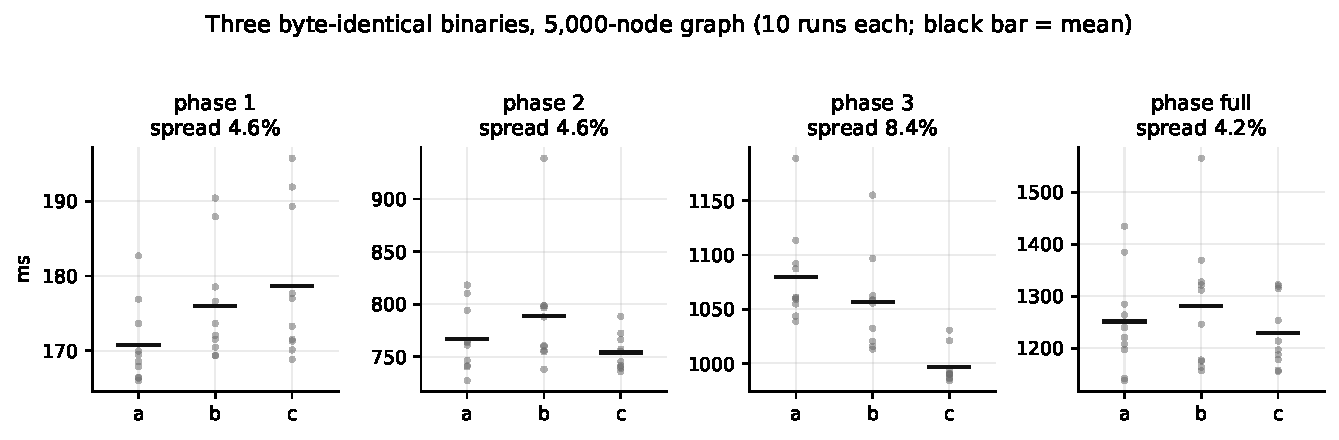
\includegraphics[width=\textwidth]{figures/fig1_null_test.pdf}
\caption{Three byte-identical binaries, 5{,}000-node graph, 10 runs each. All
spread here is ordering, thermal, and per-run variance --- the source code is
the same program. The worst case, $8.4\%$ in phase 3, is the floor we hold
claimed speedups against.}
\label{fig:null}
\end{figure}

The largest disagreement between identical programs is $8.4\%$, and we use that
conservative figure rather than the $4.2\%$ end-to-end value as the threshold
for a meaningful result. Note that this is substantially larger than the
within-command standard deviation, which is around $1.5\%$ end-to-end; reporting
only the latter would overstate confidence.

\subsection{Where baseline time goes}

Table~\ref{tab:composition} and Figure~\ref{fig:composition} give the baseline
phase composition at both graph sizes. Parsing, measured separately with
GraphViz's \texttt{gc} tool, accounts for $11.9 \pm 0.4$\,ms at 5{,}000 nodes
--- about $1\%$ of runtime --- and is included in the ranking figure below.

\begin{table}[htbp]
\centering
\caption{Baseline runtime composition, by differencing adjacent cumulative
phases. Crossing minimization dominates at 5{,}000 nodes; coordinate assignment
overtakes it at 10{,}000.}
\label{tab:composition}
\begin{tabular}{lrrrr}
\toprule
& \multicolumn{2}{c}{\textbf{5{,}000 nodes}} & \multicolumn{2}{c}{\textbf{10{,}000 nodes}} \\
\cmidrule(lr){2-3}\cmidrule(lr){4-5}
\textbf{Stage} & \textbf{ms} & \textbf{share} & \textbf{ms} & \textbf{share} \\
\midrule
Ranking                & 198.8  & 17.8\% & 214.7  & 6.2\%  \\
Crossing minimization  & 549.9  & 49.3\% & 1312.5 & 37.7\% \\
Coordinate assignment  & 252.5  & 22.6\% & 1697.6 & 48.7\% \\
Spline routing         & 114.6  & 10.3\% & 261.2  & 7.5\%  \\
\midrule
Total                  & 1115.7 & 100\%  & 3486.0 & 100\%  \\
\bottomrule
\end{tabular}
\end{table}

\begin{figure}[htbp]
\centering
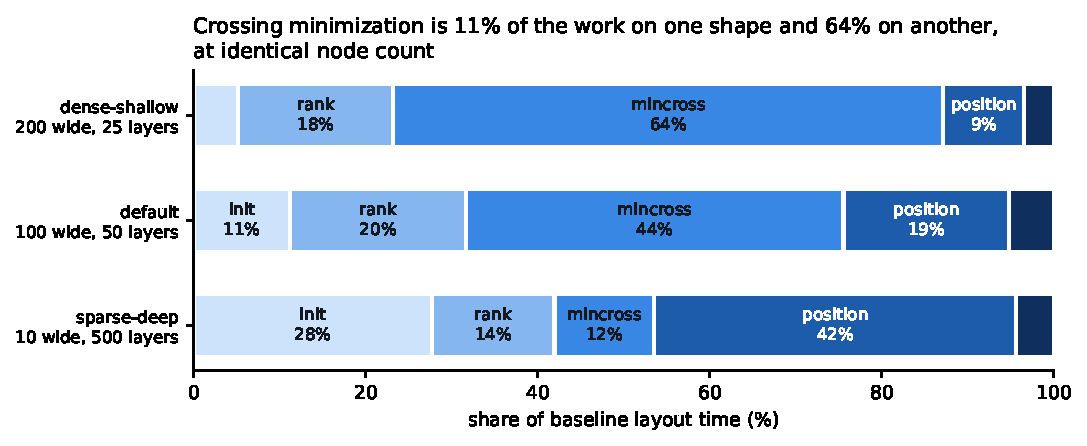
\includegraphics[width=\textwidth]{figures/fig2_phase_composition.pdf}
\caption{Baseline runtime composition at both graph sizes.}
\label{fig:composition}
\end{figure}

The shift is the important part. Crossing minimization falls from $49.3\%$ to
$37.7\%$ of runtime as the graph doubles, while coordinate assignment rises from
$22.6\%$ to $48.7\%$ and becomes dominant. Both are solved with network simplex
in the coordinate case; the crossing phase is an iterative heuristic. This
reweighting drives the divergence reported in Section~\ref{sec:scaling}.

\subsection{End-to-end results}

Table~\ref{tab:phases} gives cumulative phase timings for all three binaries at
both sizes, and Figure~\ref{fig:endtoend} plots the end-to-end result with every
individual run shown.

\begin{table}[htbp]
\centering
\caption{Cumulative phase timings, mean $\pm$ standard deviation over 10 runs.
Phases are cumulative: each row includes everything above it. All three
binaries were measured in one \texttt{hyperfine} invocation per row.}
\label{tab:phases}
\begin{tabular}{llrrr}
\toprule
\textbf{Graph} & \textbf{Phase} & \textbf{Baseline} & \textbf{Claude} & \textbf{Codex} \\
\midrule
\multirow{4}{*}{5{,}000}
 & 1 (ranking)              & $198.8 \pm 18.4$  & $184.5 \pm 14.9$  & $173.9 \pm 8.8$  \\
 & 2 (+ crossing min.)      & $748.7 \pm 27.6$  & $476.9 \pm 23.2$  & $572.9 \pm 20.1$ \\
 & 3 (+ coordinates)        & $1001.2 \pm 27.0$ & $640.2 \pm 23.7$  & $840.2 \pm 28.2$ \\
 & full (+ splines)         & $1115.7 \pm 16.2$ & $\mathbf{758.9 \pm 19.9}$ & $\mathbf{960.9 \pm 27.1}$ \\
\midrule
\multirow{4}{*}{10{,}000}
 & 1 (ranking)              & $214.7 \pm 1.4$    & $214.4 \pm 2.4$   & $221.1 \pm 11.4$  \\
 & 2 (+ crossing min.)      & $1527.2 \pm 20.0$  & $978.3 \pm 19.2$  & $1245.9 \pm 42.5$ \\
 & 3 (+ coordinates)        & $3224.8 \pm 214.1$ & $2109.1 \pm 74.7$ & $2720.6 \pm 151.9$ \\
 & full (+ splines)         & $3486.0 \pm 263.4$ & $\mathbf{2226.6 \pm 26.2}$ & $\mathbf{3028.9 \pm 292.3}$ \\
\bottomrule
\end{tabular}
\end{table}

\begin{figure}[htbp]
\centering
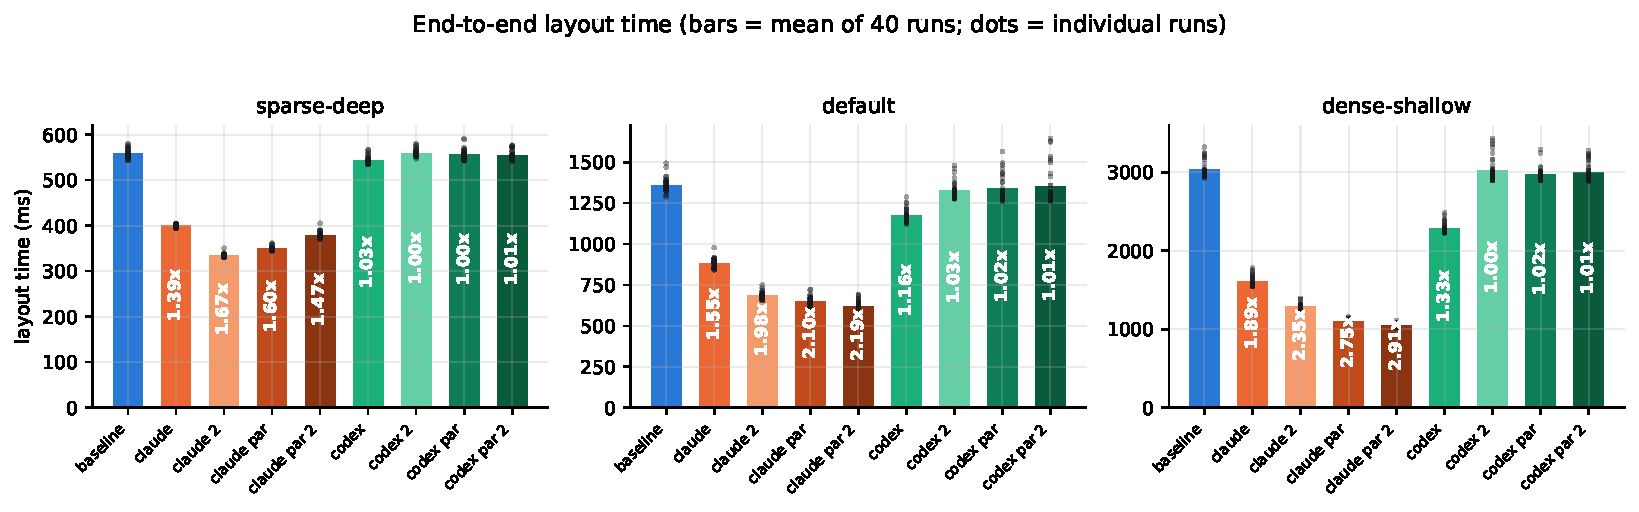
\includegraphics[width=\textwidth]{figures/fig3_end_to_end.pdf}
\caption{End-to-end layout time. Bars are means of 10 runs; dots are the
individual runs.}
\label{fig:endtoend}
\end{figure}

At 5{,}000 nodes Claude reaches $1.47\times$ and Codex $1.16\times$ end-to-end.
Both exceed the $8.4\%$ floor, Claude by a wide margin. Codex's $16\%$
improvement is roughly twice the floor: real, but a margin worth stating
explicitly rather than reporting as a bare ratio.

\subsection{Per-stage attribution}

\begin{table}[htbp]
\centering
\caption{Per-stage speedup over baseline, derived by differencing adjacent
phases. Differencing compounds the error of both terms; these are weaker
evidence than Table~\ref{tab:phases}.}
\label{tab:stages}
\begin{tabular}{lrrrr}
\toprule
& \multicolumn{2}{c}{\textbf{5{,}000 nodes}} & \multicolumn{2}{c}{\textbf{10{,}000 nodes}} \\
\cmidrule(lr){2-3}\cmidrule(lr){4-5}
\textbf{Stage} & \textbf{Claude} & \textbf{Codex} & \textbf{Claude} & \textbf{Codex} \\
\midrule
Ranking               & 1.08$\times$ & 1.14$\times$ & 1.00$\times$ & 0.97$\times$ \\
Crossing minimization & 1.88$\times$ & 1.38$\times$ & 1.72$\times$ & 1.28$\times$ \\
Coordinate assignment & 1.55$\times$ & 0.94$\times$ & 1.50$\times$ & 1.15$\times$ \\
Spline routing        & 0.97$\times$ & 0.95$\times$ & ---          & ---          \\
\bottomrule
\end{tabular}
\end{table}

Figure~\ref{fig:perrun} shows every run at 5{,}000 nodes. The ranking phase is
the cautionary case: the three binaries lie within about 25\,ms of one another
on a measurement whose per-binary standard deviation is 9--18\,ms, and their
distributions overlap almost completely. We report ranking as no difference.
Neither agent modified the ranking path in a way that would be expected to
matter here, since the generated graphs pin ranks explicitly and leave little
ranking work to do.

Spline routing at 10{,}000 nodes is omitted from Table~\ref{tab:stages}. It is
derived by subtracting two quantities whose standard deviations are 214\,ms and
263\,ms, and the resulting figure is not meaningful.

\begin{figure}[htbp]
\centering
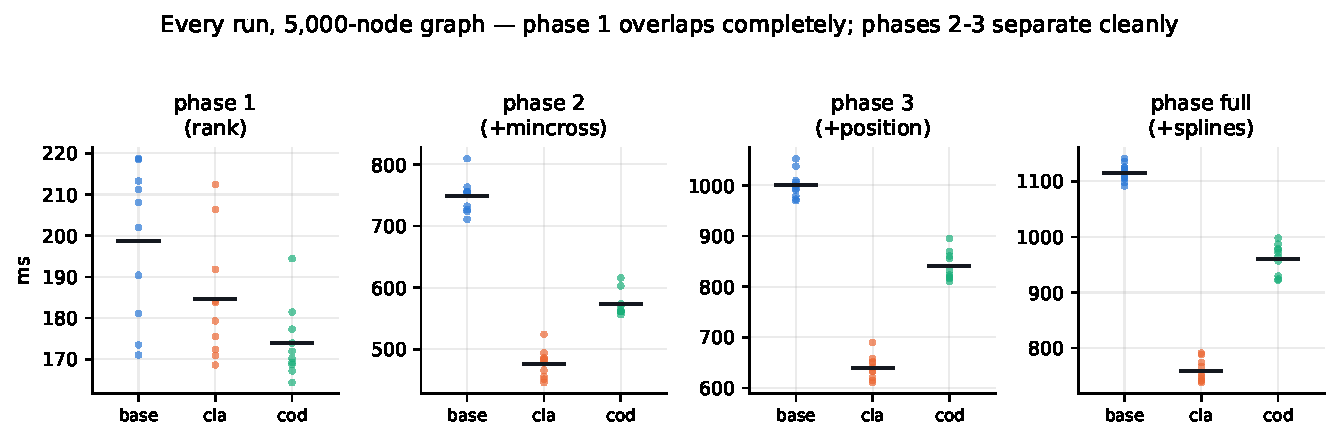
\includegraphics[width=\textwidth]{figures/fig4_per_run_distributions.pdf}
\caption{All 10 runs per binary per phase, 5{,}000-node graph. The ranking
phase overlaps completely across all three binaries; phases 2 and 3 separate
cleanly.}
\label{fig:perrun}
\end{figure}

\subsection{Scaling}
\label{sec:scaling}

\begin{figure}[htbp]
\centering
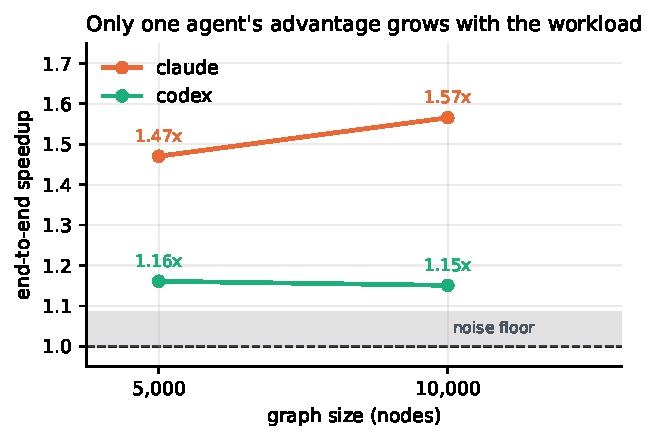
\includegraphics[width=0.62\textwidth]{figures/fig5_scaling.pdf}
\caption{End-to-end speedup against graph size, with the noise floor shaded.
Two points are suggestive, not a fitted trend.}
\label{fig:scaling}
\end{figure}

Doubling the graph separates the two agents (Figure~\ref{fig:scaling}). Claude
improves from $1.47\times$ to $1.57\times$; Codex is flat, $1.16\times$ to
$1.15\times$. Table~\ref{tab:stages} shows the mechanism: at 10{,}000 nodes
coordinate assignment is $48.7\%$ of runtime, and Claude achieves $1.50\times$
on it against Codex's $1.15\times$.

\subsection{What the agents changed}

Both agents modified crossing minimization, and both arrived independently at
the same core idea: the two symmetric crossing-count computations for an
adjacent node pair can be fused into a single pass, since any pair of incident
edges contributes to at most one of the two counts.

\textbf{Codex} made two code commits touching only
\texttt{lib/dotgen/mincross.c} (+122/$-$17 lines). Beyond the fused counts, it
replaced a linear prefix scan in the crossing-count routine with a Fenwick tree,
reducing that inner loop from $O(n)$ to $O(\log n)$.

\textbf{Claude} made eight code commits touching
\texttt{lib/dotgen/mincross.c} and \texttt{lib/common/ns.c} (+978/$-$169 lines).
It found the same fused-count transformation, then restructured the network
simplex implementation: the depth-first traversal keeps its current frame in
local variables backed by a reusable stack, and the scattered per-node fields
reached through accessor macros were replaced by a dense 32-byte-per-node state
array with cached neighbour pointers. This is a memory-locality change, and it
is what produces the coordinate-assignment improvement in
Table~\ref{tab:stages}.

\subsection{Correctness}

Both agents' binaries produce \texttt{dot -Tdot} output byte-identical to the
baseline on the evaluation graphs (SHA-1 \texttt{3560c5d0\ldots} at 5{,}000
nodes). We read both diffs against the prompt's list of disallowed shortcuts and
found no reduced iteration counts, early exits, input special-casing, or
modified tests. Neither diff contains any OpenMP directive, thread creation, or
other concurrency construct.

\section{Discussion}
\label{sec:discussion}

\subsection{Both agents found the bottleneck; only one kept going}

Neither agent was told where to look, and both went to crossing minimization.
Working in isolation, both arrived at the same transformation: fusing the two
symmetric crossing-count passes. Locating the expensive phase is evidently not
the hard part.

What separates them is how far they went next. Codex stopped at the phase it
identified. Claude continued into network simplex, which serves both ranking and
coordinate assignment, and that accounts for its entire margin --- the same
pattern on three workloads with very different composition, not an inference
from one measurement.

\subsection{Why breadth mattered: the ceiling moves with shape}

Amdahl's law~\cite{amdahl1967validity} bounds what optimizing one phase can
yield, and that bound depends on the phase's share of runtime --- which
Table~\ref{tab:composition} shows is a property of the graph's shape.

\begin{table}[htbp]
\centering
\caption{What optimizing crossing minimization alone can achieve, against what
each agent measured. \textbf{Ceiling:} baseline wall clock divided by (wall
clock minus that phase's measured cost), i.e.\ the phase driven to zero.
\textbf{Claude and Codex:} the end-to-end speedups from
Table~\ref{tab:endtoend}, carrying the same dagger convention.}
\label{tab:ceiling}
\begin{tabular}{lrrr}
\toprule
\textbf{Graph} & \textbf{Ceiling, crossing min.\ only} & \textbf{Claude} & \textbf{Codex} \\
\midrule
sparse-deep   & 1.11$\times$ & \textbf{1.33$\times$} & 0.99$\times$$^\dagger$ \\
default       & 1.69$\times$ & 1.50$\times$ & 1.16$\times$ \\
dense-shallow & 2.58$\times$ & 1.84$\times$ & 1.29$\times$ \\
\bottomrule
\end{tabular}
\end{table}

Codex sits below the ceiling on all three shapes, as an agent that optimized
only that phase must. On sparse-deep the ceiling is $1.11\times$, so even a
perfect crossing-minimization optimization would be nearly invisible end-to-end.
Codex's $0.99\times$ is not a failed optimization --- it works, at $1.31\times$
on the phase --- but a phase worth $11.5\%$ of the workload.

Claude \emph{exceeds} that ceiling, $1.33\times$ against $1.11\times$, which is
only possible by improving other phases. That is the breadth argument at its
sharpest: on that workload no amount of further work on the phase both agents
found could have matched it.

The ceiling an optimization can reach is a property of the input, not the
program, and a single benchmark graph cannot show that.

\subsection{Cost}

\begin{table}[H]
\centering
\caption{Claude run cost, as reported by its session log.}
\label{tab:cost-claude}
\begin{tabular}{lr}
\toprule
\textbf{Metric} & \textbf{Value} \\
\midrule
Model                 & \texttt{claude-opus-5} \\
Working time          & 4\,h\,27\,m\,3\,s \\
\midrule
Input tokens          & 730 \\
Output tokens         & 620,448 \\
Cache creation tokens & 1,270,669 \\
Cache read tokens     & 89,851,473 \\
\midrule
Total tokens          & 91,743,320 \\
\bottomrule
\end{tabular}
\end{table}

\begin{table}[H]
\centering
\caption{Codex run cost, as reported by its session log. Cached input is a
subset of input; reasoning output is a subset of output.}
\label{tab:cost-codex}
\begin{tabular}{lr}
\toprule
\textbf{Metric} & \textbf{Value} \\
\midrule
Model                     & \texttt{gpt-5.6-terra} \\
Working time              & 23\,m\,42\,s \\
\midrule
Input tokens              & 5,114,035 \\
\quad Cached input tokens & 4,985,600 \\
Output tokens             & 20,826 \\
\quad Reasoning tokens    & 4,555 \\
Cache-write tokens        & 0 \\
\midrule
Total tokens              & 5,134,861 \\
\bottomrule
\end{tabular}
\end{table}

\section{Limitations}
\label{sec:limitations}

We state these plainly because several of them bound the conclusions above.

\paragraph{One run per agent.}
Each agent was invoked once. Agent behaviour is stochastic, so we cannot say
whether the ordering we observed is stable or whether a second invocation of
either would find a different target. This is the single weakest point in the
study, and it means our results describe two particular runs rather than two
systems.

\paragraph{Synthetic graphs only.}
All three shapes come from the same generator, which produces uniform rank
widths and constant fanout. Real inputs to \texttt{dot} are irregular in both.
A generator also encodes assumptions about the workload that do not show up in
aggregate timings, and we cannot rule out ones we have not noticed.

\section*{Reproducibility Statement}
\label{sec:repro}

Every number in this paper comes from data in the artifact below. No result is
estimated, extrapolated, or reported from a source other than the raw
measurement files.

\paragraph{Artifacts.}
\begin{itemize}
\item Claude's diff and commit history: \\
      \url{https://github.com/harvest7777/claude-graphviz-run/compare/main...agent-work}
\item Codex's diff and commit history: \\
      \url{https://github.com/harvest7777/codex-graphviz-run/compare/main...agent-work}
\item Raw timing data and session dumps: \\
      \url{https://github.com/harvest7777/graphviz-results-dump}
\end{itemize}

\paragraph{Source.}
GraphViz at commit
\texttt{23b06521ab916e7f4f2ae2f9ef8413a8ccc66601}, from
\url{https://gitlab.com/graphviz/graphviz.git}. Both agent branches are named
\texttt{agent-work} and branch from that commit.

\paragraph{Build.}
\begin{verbatim}
cmake -S <sandbox> -B <build> \
  -DCMAKE_INSTALL_PREFIX=<prefix> \
  -DWITH_POPPLER=OFF -DWITH_GVEDIT=OFF \
  -DCMAKE_BUILD_TYPE=Release
cmake --build <build> -j12 && cmake --install <build>
\end{verbatim}
Identical for all three sandboxes. On macOS a Bison $\geq 3.0$ path must be
passed explicitly, as the system Bison is too old for the GraphViz build.

\paragraph{Measurement.}
\texttt{hyperfine} 1.20.0, 10 warmup and 10 timed runs, all binaries for a given
(graph, phase) in a single invocation. Graphs are produced by the fixed-seed
generator in the artifact repository. Raw per-run timings for every
configuration --- including the null test --- are in the results repository as
\texttt{hyperfine} JSON exports.

\paragraph{Figures.}
Every figure is regenerated from the raw JSON by a single script in the artifact
(\texttt{figures/make\_figures.py}).

\paragraph{Environment.}
Apple M4 Pro, 12 cores (8 performance, 4 efficiency), 24\,GB unified memory,
macOS 26.5.2, Apple Clang 17.0.0.

\paragraph{Agents.}
\texttt{claude-opus-5} (Claude Code) and \texttt{gpt-5.6-terra} (Codex), each
invoked once, autonomously, with the prompt reproduced in the artifact
repository. Neither had network access to the evaluation harness or benchmark
graphs.

\section{Conclusion}
\label{sec:conclusion}

Two coding agents, given an identical checkout of GraphViz and a prompt naming
no target, both located the dominant cost in the \texttt{dot} layout pipeline
and produced output-preserving speedups: $1.47\times$ and $1.16\times$
end-to-end at 5{,}000 nodes, against an $8.4\%$ measured noise floor. Finding
the bottleneck was evidently not the difficult part of the task.

What separated them was scope. At 10{,}000 nodes the dominant phase shifts from
crossing minimization to coordinate assignment, and the agent that had
restructured network simplex --- code shared by both phases --- improves to
$1.57\times$ while the agent that optimized a single function stays flat at
$1.15\times$. An optimization's value depends on whether the phase it targets
grows or shrinks with the workload, and a single problem size cannot reveal
that.

Neither agent used parallelism. On this workload the ceiling arithmetic suggests
that was the right call: at 10{,}000 nodes, idealized eight-core parallelization
of crossing minimization caps end-to-end speedup at $1.49\times$, and one agent
exceeded that serially at $1.57\times$ --- without introducing concurrency or the
possibility of a race.

The results are modest, and we have tried to report them at the size they
actually are. The protocol may be the more durable contribution: measure the
noise floor with byte-identical binaries before measuring anything else, hold
the evaluation harness out of the agents' reach, forbid the shortcuts that
manufacture speedups, and attribute results by phase at more than one problem
size. Each of these caught something in this study that a simpler design would
have reported as a finding.

Immediate future work is to repeat both agent runs to establish whether the
ordering is stable, extend to a third graph size and to non-layered topologies,
and complete the correctness checks named in Section~\ref{sec:limitations}.


\bibliographystyle{plain}
\bibliography{references}

\end{document}
